
\section{Controlling an LED using Pushbutton}
\subsection{Introduction}
Controlling an LED using a pushbutton is a fundamental experiment 
that demonstrates digital input and output
interaction in microcontrollers.
In this setup, an external pull-down resistor
is used with the pushbutton to ensure a stable
and defined logic level when the button is not pressed.
When the button is open, the resistor keeps the input pin
at a LOW (0V) state, and when the button is pressed,
the pin reads HIGH (3.3V or 5V, depending on 
the microcontroller logic).

The STM32F103C6 microcontroller allows us to easily read the state
of a pushbutton using digital input pins and control 
an LED output pin accordingly.
In the Arduino framework, the \texttt{digitalRead}
function is used to detect the button press,
and the \texttt{digitalWrite} function is used to
turn the LED ON or OFF based on the button's state.
This experiment helps in understanding how external
components like switches interface with microcontroller
GPIOs and how pull-down resistors prevent floating inputs,
ensuring reliable operation of the circuit.
\subsection{Procedure}
\begin{enumerate}
  \item I have collected a microcontroller STM32 blue pill, STLink programmer,
    a breadboard, an LED, a $220\Omega$ resistor, a pushbutton, a $10k\Omega$ resistor (for pull-down), and some jumper wires.
  \item Connected the LED's anode pin to GPIO pin PB0 through the $220\Omega$ resistor, 
    and connected the LED's cathode to ground.
  \item Connected one terminal of the pushbutton to 3.3V ($V_{cc}$), and the other terminal to GPIO pin PC15.
  \item Connected a $10k\Omega$ resistor between PC15 and ground to serve as the pull-down resistor.
  \item Written the code to turn the LED ON when the button is pressed and OFF when it is released (see code~\ref{code:pushbutton}), and uploaded it using the STLink programmer.
\end{enumerate}
\newpage
\subsection{Diagram}
\begin{figure}[htbp]
    \centering
    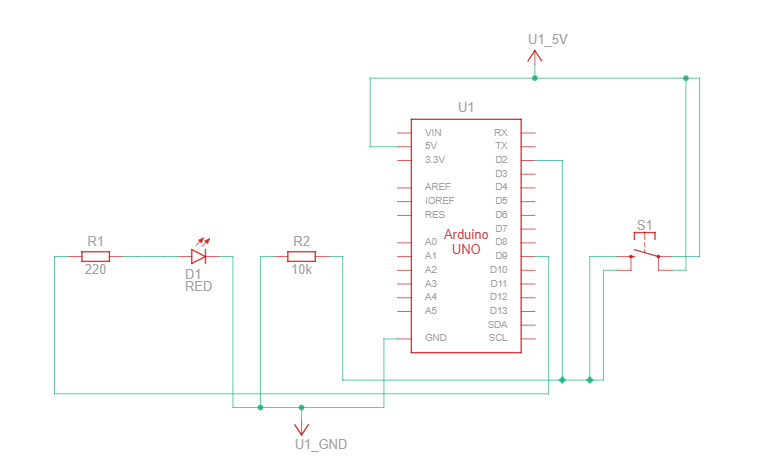
\includegraphics[width=0.8\textwidth]{img/pushbtn.png}
    \caption{Schematic diagram of the circuit using Arduino in TinkerCAD}\label{fig:sim}
\end{figure}
\subsection{Source Code}
\begin{code}
\caption{Controlling an LED using pushbutton}
\begin{minted}[frame=single, linenos]{cpp}
#include <Arduino.h>
const int LED = PB0;
// The LED is connected to pin 9
const int BUTTON = PC15;
// The Button is connected to pin 2
void setup(){
  pinMode(LED, OUTPUT);
  pinMode(BUTTON, INPUT);
}
void loop(){
  if (digitalRead(BUTTON) == HIGH){
    digitalWrite(LED, LOW);
  } else {
    digitalWrite(LED, HIGH);
  }
}
\end{minted}
    \label{code:pushbutton}
\end{code}

\section{Discussion}

Through this project, I have learned how to interface a pushbutton with the STM32F103C6 microcontroller using an external pull-down resistor. I understood the purpose of the pull-down resistor in preventing floating inputs and ensuring reliable detection of button presses.
By reading the pushbutton state and controlling the LED accordingly, I gained practical experience with digital input and output in embedded systems.
